\documentclass{beamer}

% Theme and Color Scheme
\usetheme{Boadilla}
\usecolortheme{seahorse}
\setbeamersize{text margin left=0.5cm, text margin right=0.5cm}
\setbeamertemplate{footline}{} % Remove footer
\date{}

% Required Packages
\usepackage{graphicx} % For including images
\usepackage{amsmath}  % For advanced math environments
\usepackage{amssymb}
\usepackage{booktabs} % For professional tables
\usepackage[authoryear,round]{natbib} % switched to author–year citations
\usepackage{qrcode} % For QR codes
\usepackage{listings} % nicer, line-wrapping code
\lstset{
  basicstyle=\ttfamily\scriptsize,
  breaklines=true,
  showstringspaces=false,
  columns=fullflexible,
  upquote=true
}
\usepackage{tikz}
\usetikzlibrary{positioning,arrows.meta,fit,calc,shadows.blur}

% Title Page Information
\title[RMSTSS]{RMSTSS: A Comprehensive Software Suite for Power and Sample Size Calculation in Modern Clinical Trials}
\author{Arnab Aich}
\institute{Florida State University}
\date{\today}

\begin{document}

% Frame 1: Title Page
\begin{frame}
  \titlepage
\end{frame}

% --- Part 1: Introduction & Foundations ---

% Frame 2: The Fundamental Goal of this Project
% ---------- Revised Intro Slide ----------
\begin{frame}
\frametitle{The Fundamental Goal: Planning Better Clinical Trials}

\begin{block}{Two Questions Every Trial Must Answer}
\begin{enumerate}
  \item How many participants are needed? \textbf{(sample size)}
  \item What is the chance of detecting a true effect?\textbf{(power)}
\end{enumerate}
\end{block}

\vspace{0.6em}

\begin{block}{Why This Matters}
\begin{itemize}
  \item \textbf{Ethics:} Avoid underpowered or unnecessary studies.
  \item \textbf{Efficiency:} Trials are costly—careful design saves time and resources.
  \item \textbf{Science:} Adequate power is essential for trustworthy conclusions.
\end{itemize}
\end{block}

\end{frame}
% Frame 3: The Standard Approach: Survival Models
\begin{frame}
\frametitle{The Standard Approach: Survival Models}
In many trials, the outcome is the \textbf{time until an event} occurs (e.g., recovery, disease progression, death).

\begin{block}{Key Notations}
\begin{itemize}
    \item $T$: The true time-to-event for a subject.
    \item $C$: The censoring time (e.g., end of study, patient drops out).
    \item We observe $Y = \min(T, C)$ and an event indicator $\delta$.
    \item \textbf{Survival Function}, $S(t) = P(T > t)$: The probability of surviving past time $t$.
    \item \textbf{Hazard Function}, $h(t)$: The instantaneous risk of the event at time $t$, given survival up to $t$.
    $$h(t) = \lim_{\Delta t \to 0} \frac{P(t \le T < t + \Delta t \mid T \ge t)}{\Delta t} = \frac{f(t)}{S(t)}$$
\end{itemize}
\end{block}
\end{frame}

% Frame 4
\begin{frame}
\frametitle{Proportional Hazards (PH) and Hazard Ratio Issues}

\begin{columns}[T,onlytextwidth]
  %%% Left column: Assumption + image %%%
  \begin{column}{0.48\textwidth}
    \begin{block}{PH Assumption}
      Treatment hazard is a constant multiple of control:
      \[
        h_1(t) = h_0(t)\cdot \theta
      \]
    \end{block}

    \centering
    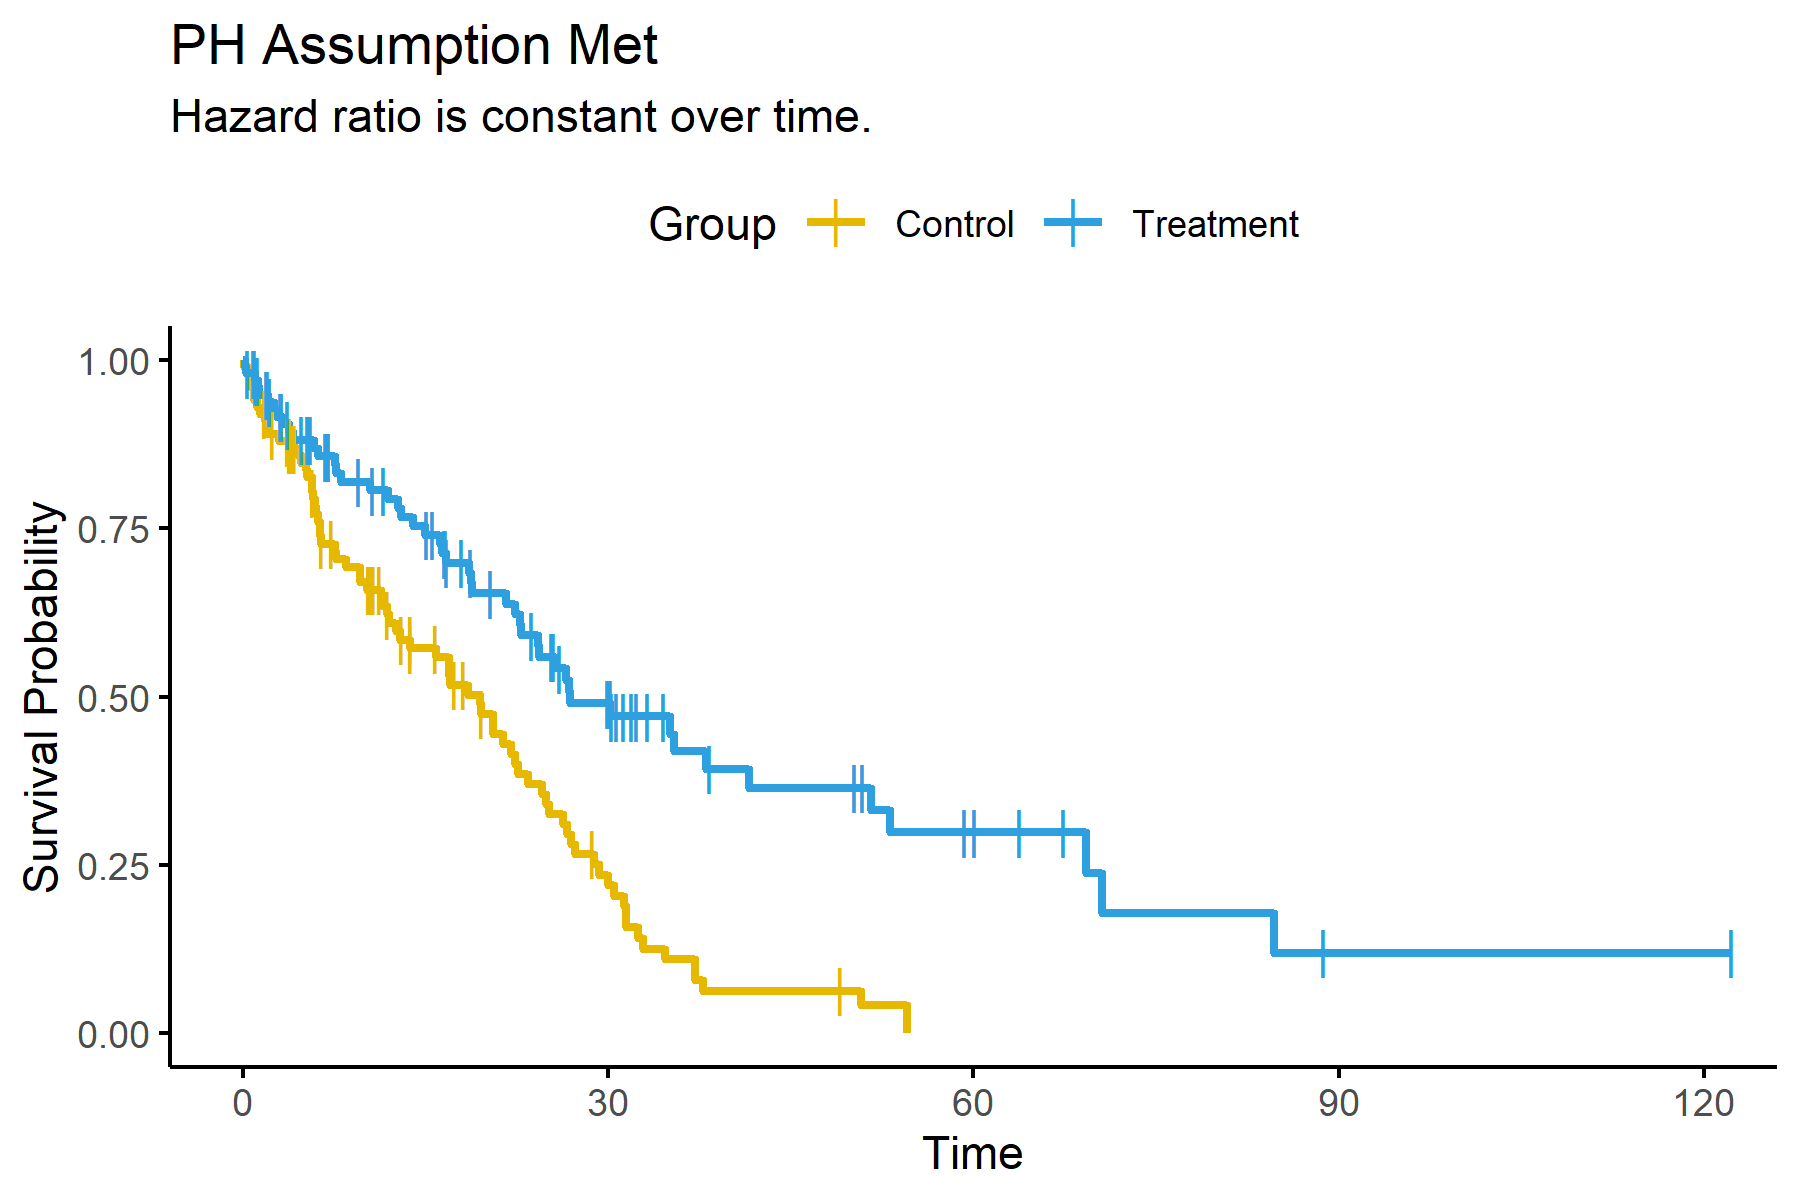
\includegraphics[width=\linewidth,height = 0.9\linewidth]{images/ph_assumption_met.png} \\
  \end{column}

  \hspace{0.04\textwidth}

  %%% Right column: Problems + image %%%
  \begin{column}{0.48\textwidth}
    \begin{block}{Problems with HR}
      \begin{itemize}
        \item PH often fails (delayed effects, waning benefit, crossing curves).
        \item No Causal interpretation.
      \end{itemize}
    \end{block}
    \centering
    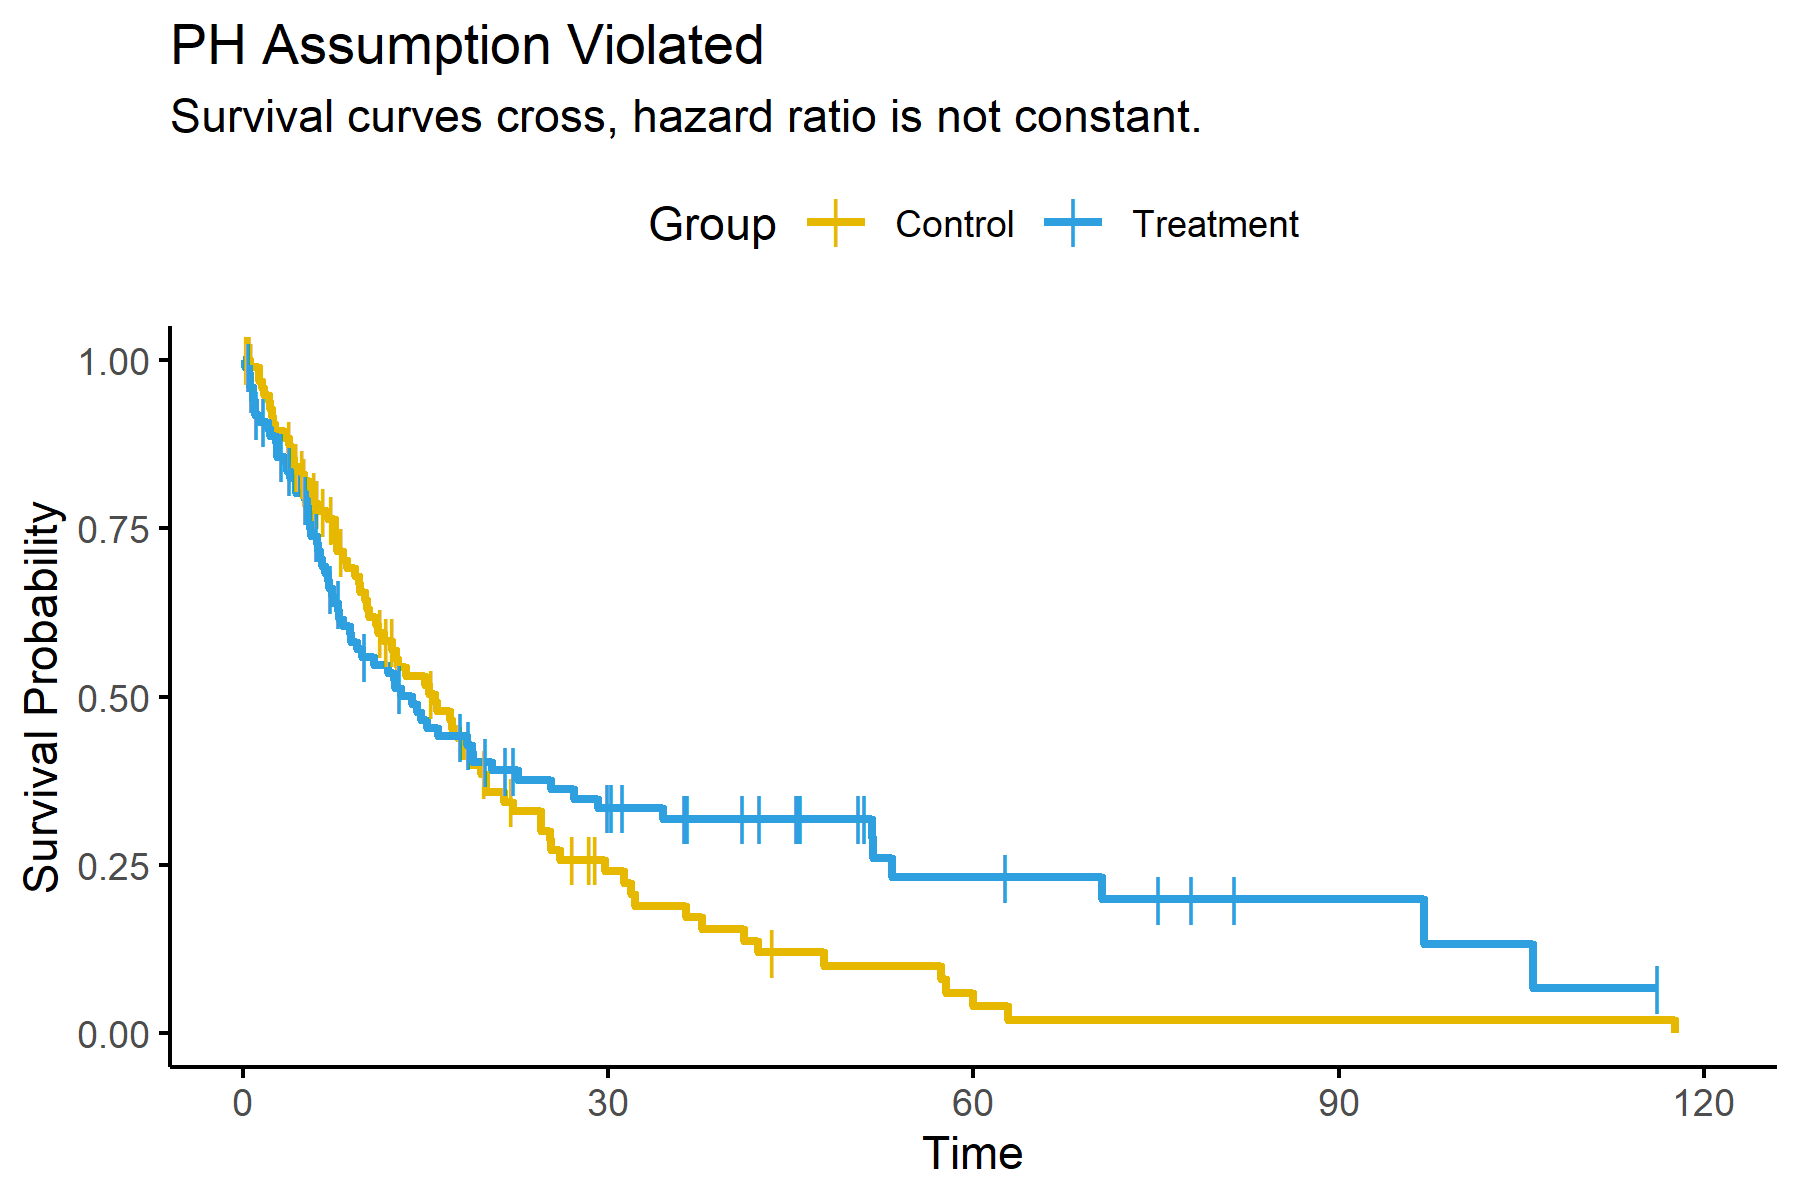
\includegraphics[width=\linewidth,height = 0.9\linewidth]{images/ph_assumption_violated.png} \\
  \end{column}
\end{columns}

\end{frame}



% Frame 5
\begin{frame}
\frametitle{The Solution: Restricted Mean Survival Time (RMST)}
\begin{block}{Definition}
The RMST is the average event-free survival time up to a pre-specified time point, $L$. It is the area under the survival curve from 0 to $L$.
$$\mu(L) = E[\min(T, L)] = \int_0^L S(t) dt$$
\end{block}

\begin{block}{Interpretation \& Advantages}
\begin{itemize}
    \item \textbf{Directly Interpretable:} It provides a clear, absolute measure of survival in units of time.
    \item \textbf{No Proportional Hazards Assumption:} The RMST is a non-parametric measure, making it a valid and robust choice even when survival curves cross.
    \item \textbf{Clinically Meaningful:} It quantifies the average time gained or lost, which is highly relevant to both clinicians and patients.
\end{itemize}
\end{block}
\end{frame}

% Merged causal interpretation slide

\begin{frame}
\frametitle{Causal Interpretation of RMST Difference}

% Top block: formula + interpretation
\begin{block}{}
\[
\Delta(L) = \mu_{\text{treat}}(L) - \mu_{\text{control}}(L)
\]

\begin{itemize}
  \item $\Delta(L)$ quantifies the \textbf{average gain in event-free time} from treatment over $[0,L]$.  
  \item Interpreted directly in \textbf{time units} (e.g., “3 extra months without progression”).  
  \item The treatment effect is the \textbf{difference in area under the survival curves} up to $L$.  
\end{itemize}
\end{block}

% Bottom row: two images, no titles/captions
\begin{columns}[T,onlytextwidth]
  \begin{column}{0.5\textwidth}
    \centering
    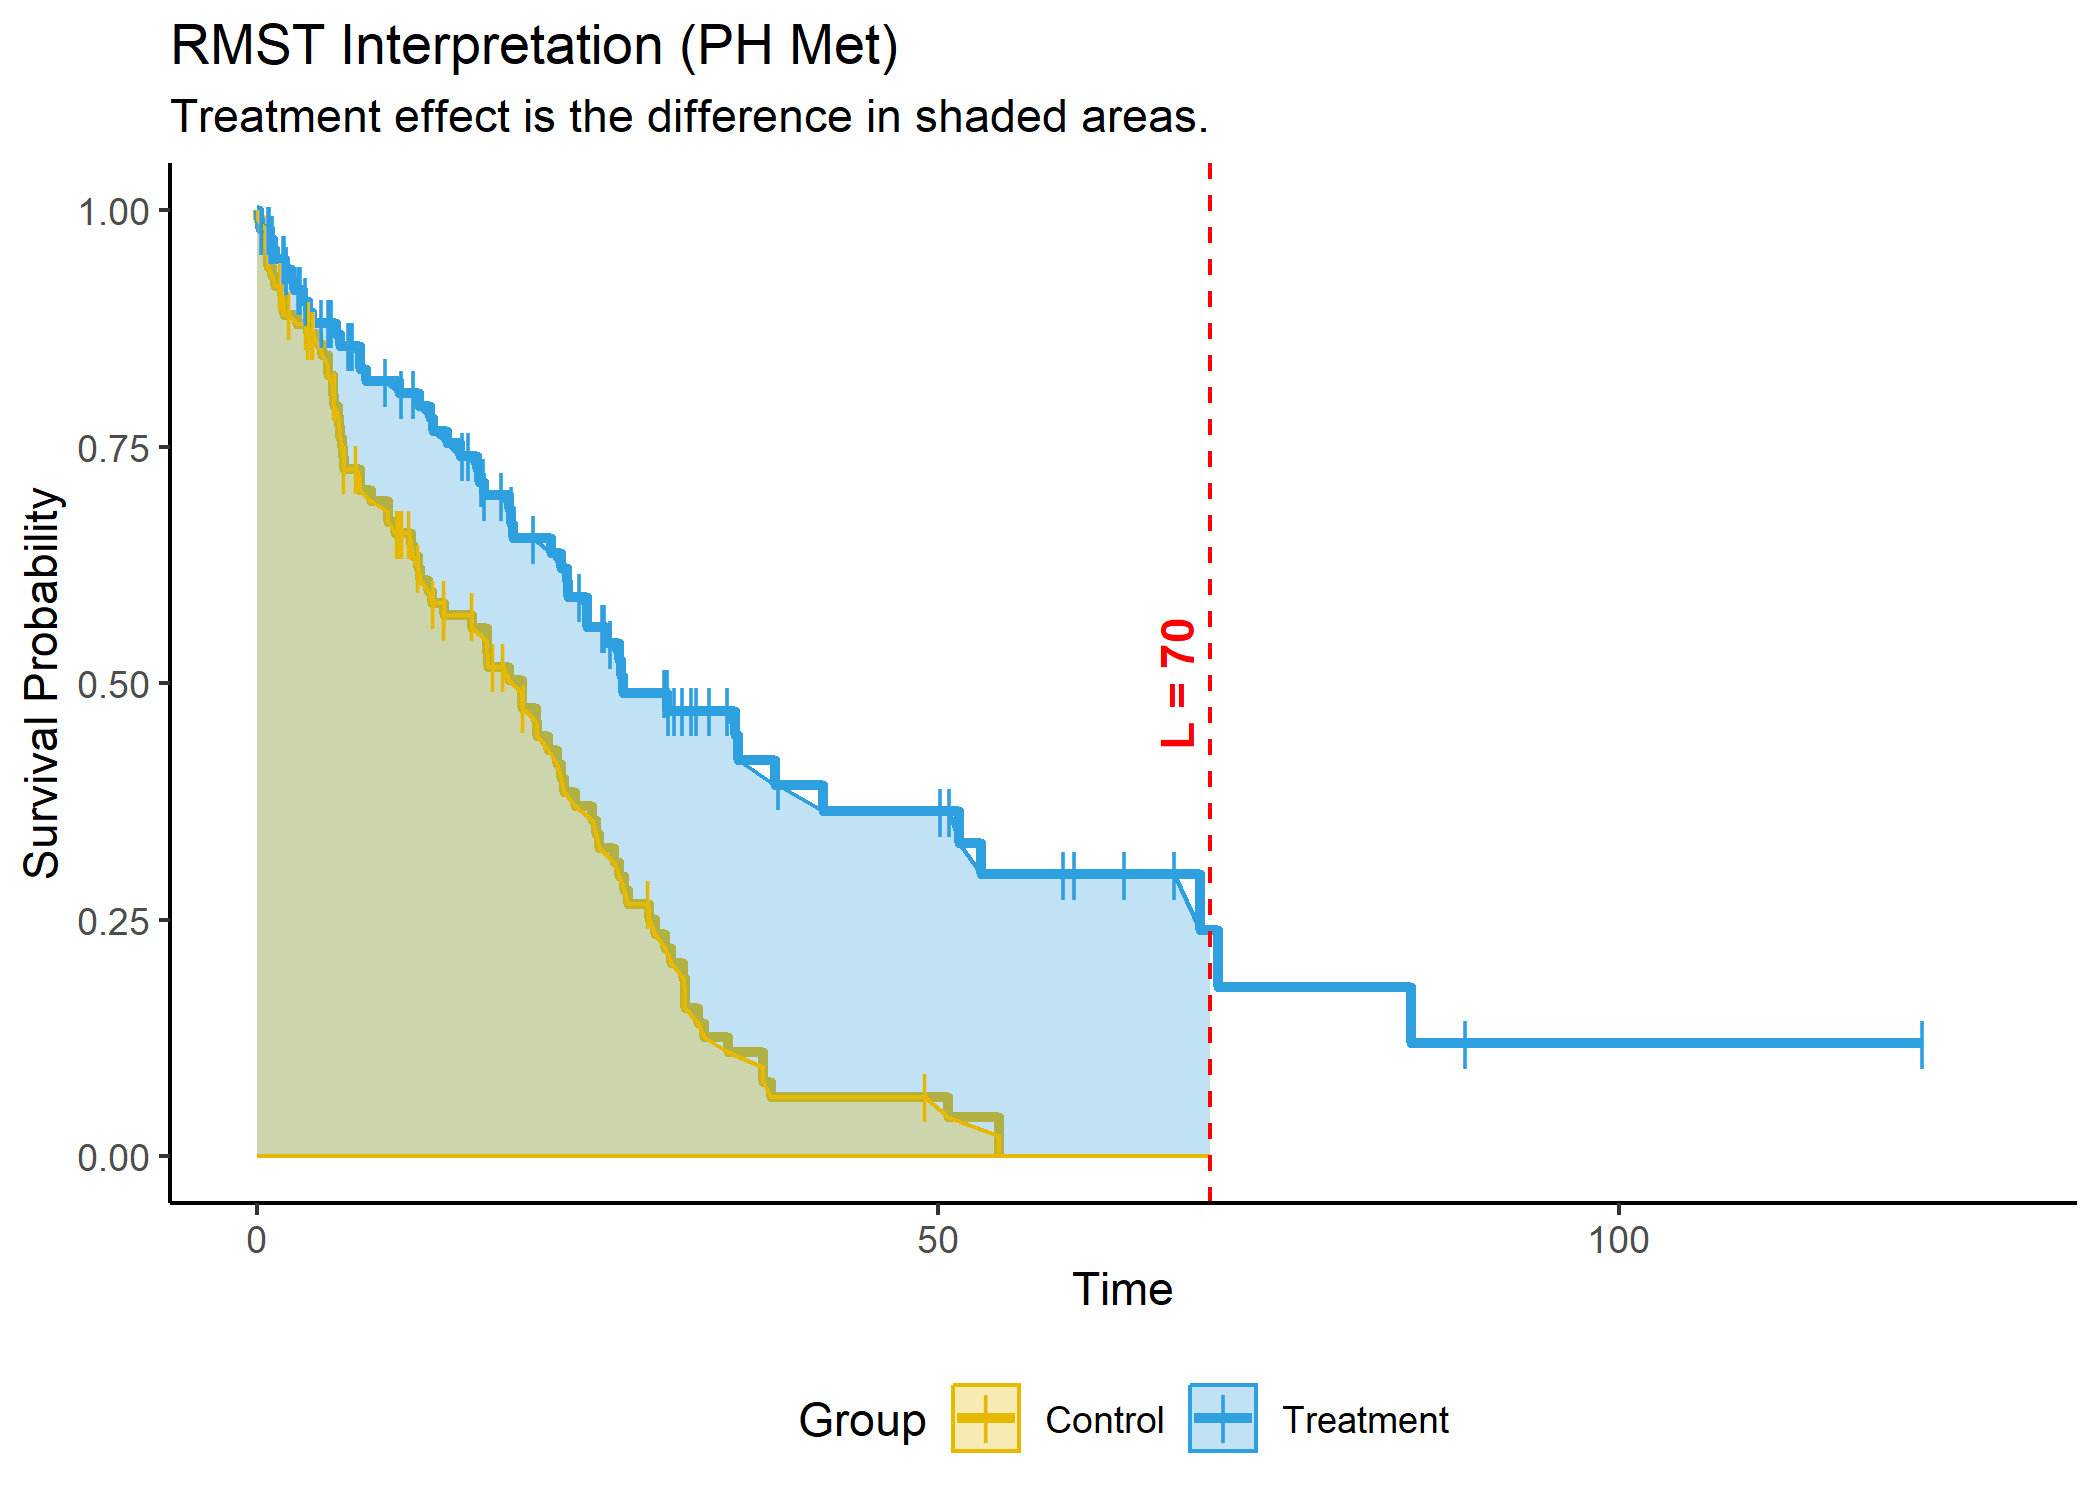
\includegraphics[width=\textwidth, height=0.7\textwidth]{images/rmst_causal_plot_ph_met.png}
  \end{column}
  \begin{column}{0.5\textwidth}
    \centering
    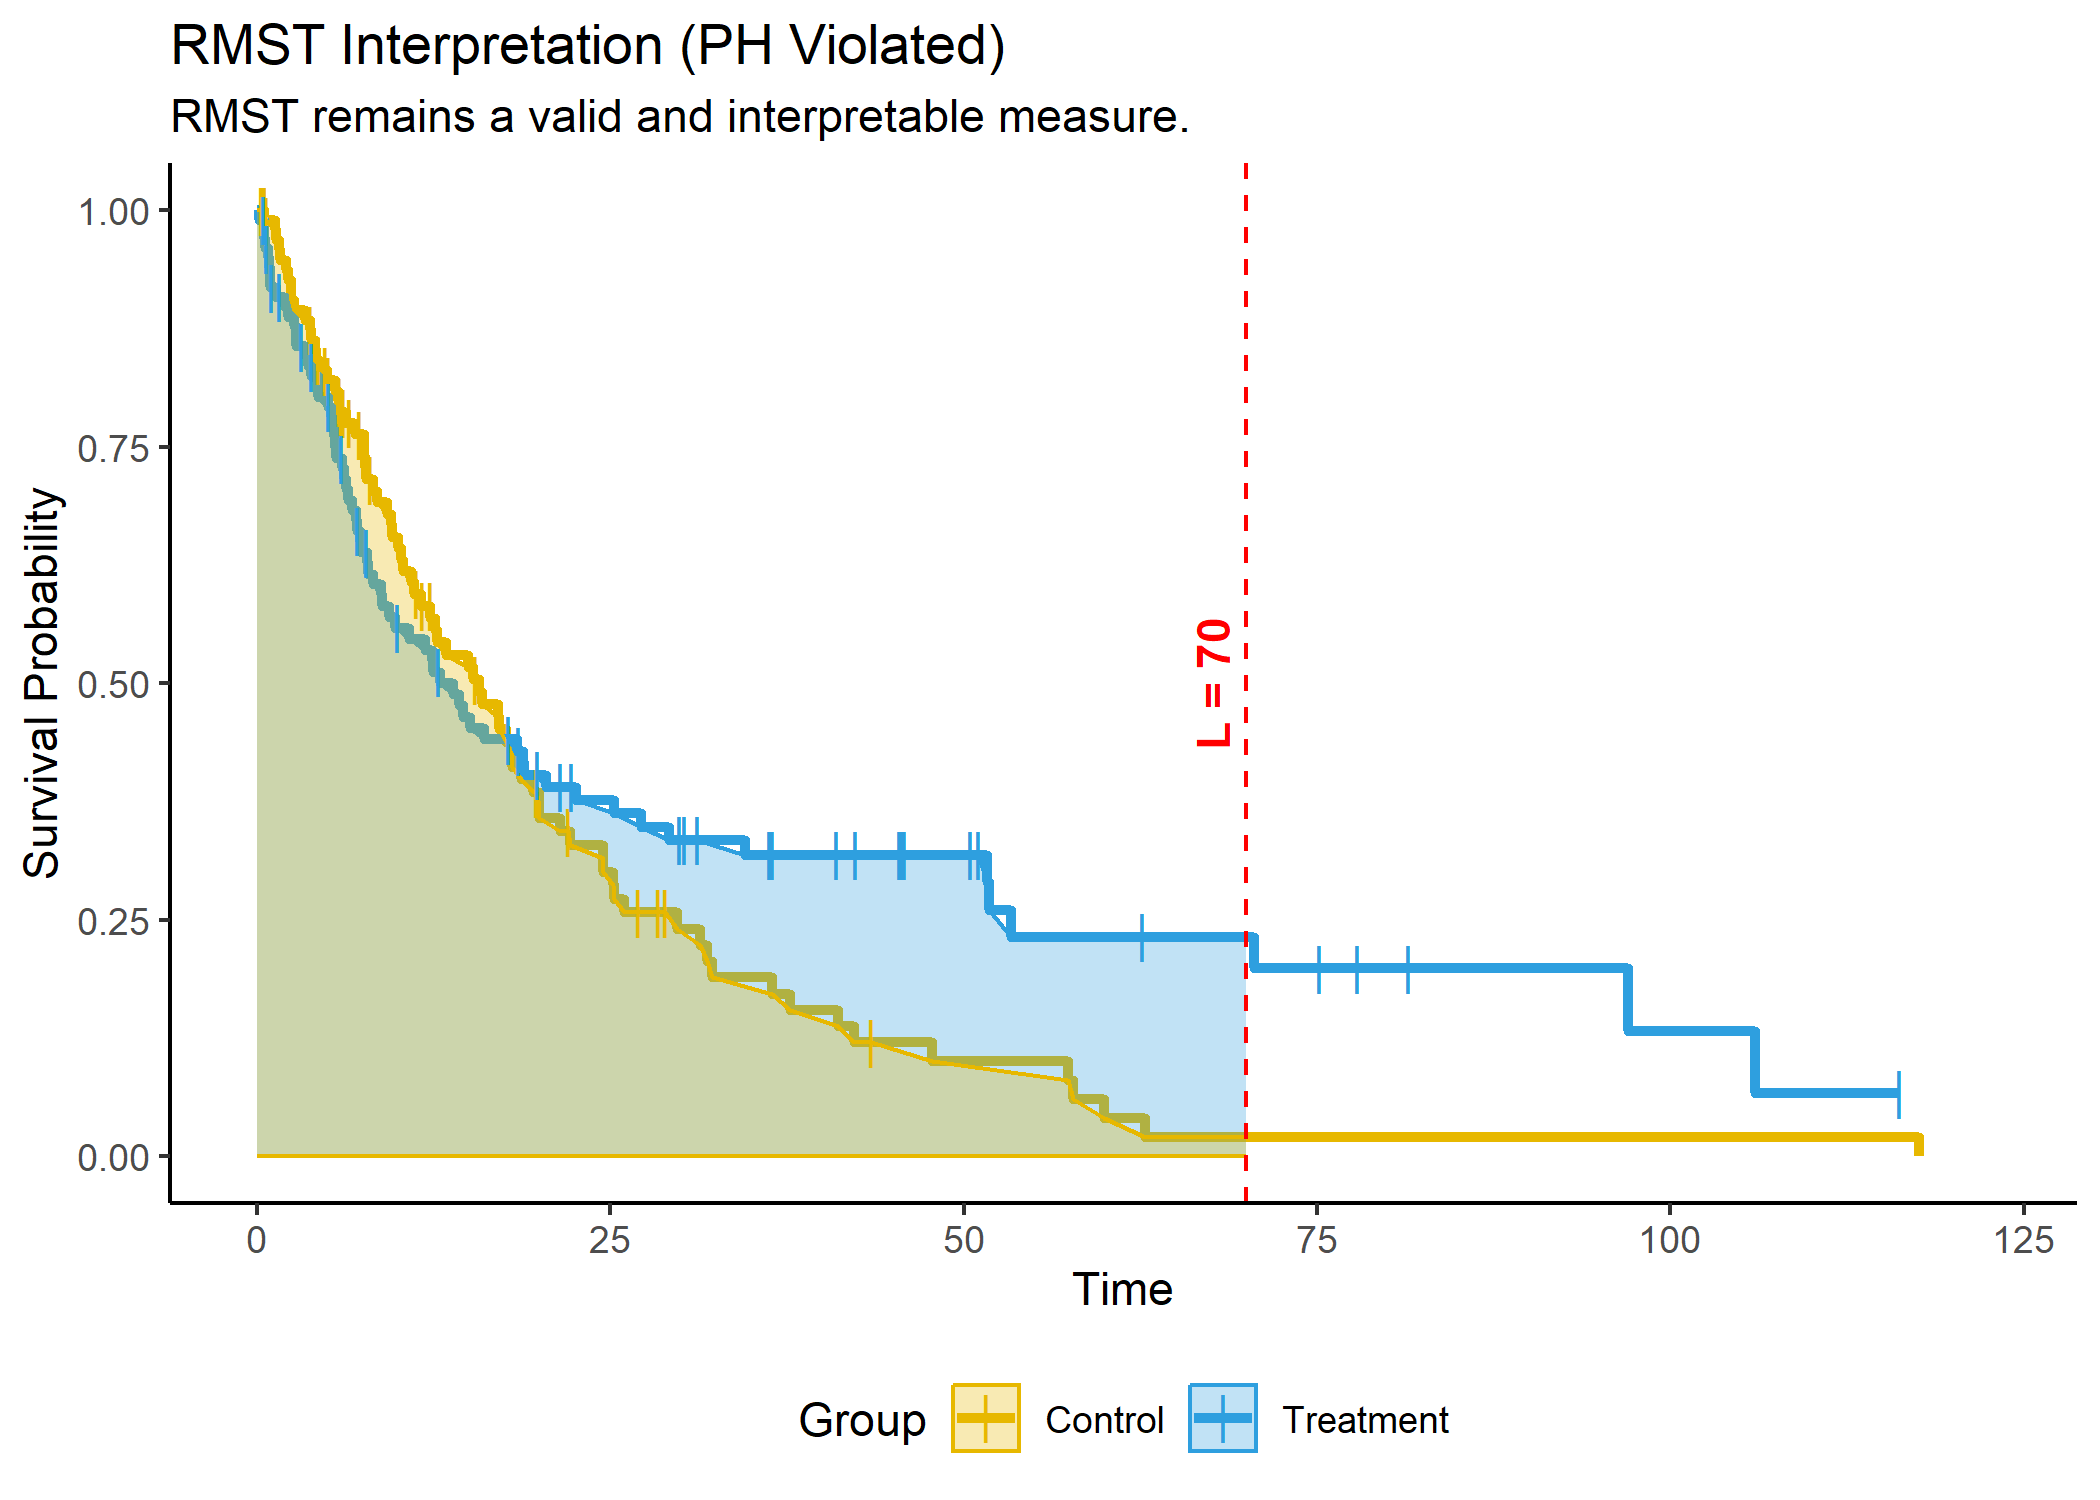
\includegraphics[width=\textwidth, height=0.7\textwidth]{images/rmst_causal_plot_ph_violated.png}
  \end{column}
\end{columns}

\end{frame}



% --- Part 2: The RMSTSS Package: Models & Methods ---



% ---------- New Slide: Our Contributions ----------
\begin{frame}
\frametitle{Bridging Gap: Theory and Implementation}

\begin{block}{We Provide:}
\scriptsize
\begin{itemize}
  \item Unified framework for \textbf{RMST-based power and sample size} calculations.
  \item \textbf{RMSTSS R package}: open-source, reproducible implementation.
  \item \textbf{RMSTSS Shiny web app}: user-friendly interface, no coding required.
\end{itemize}
\end{block}
\textit{The following models are currently available.}
\begin{figure}
    \centering
    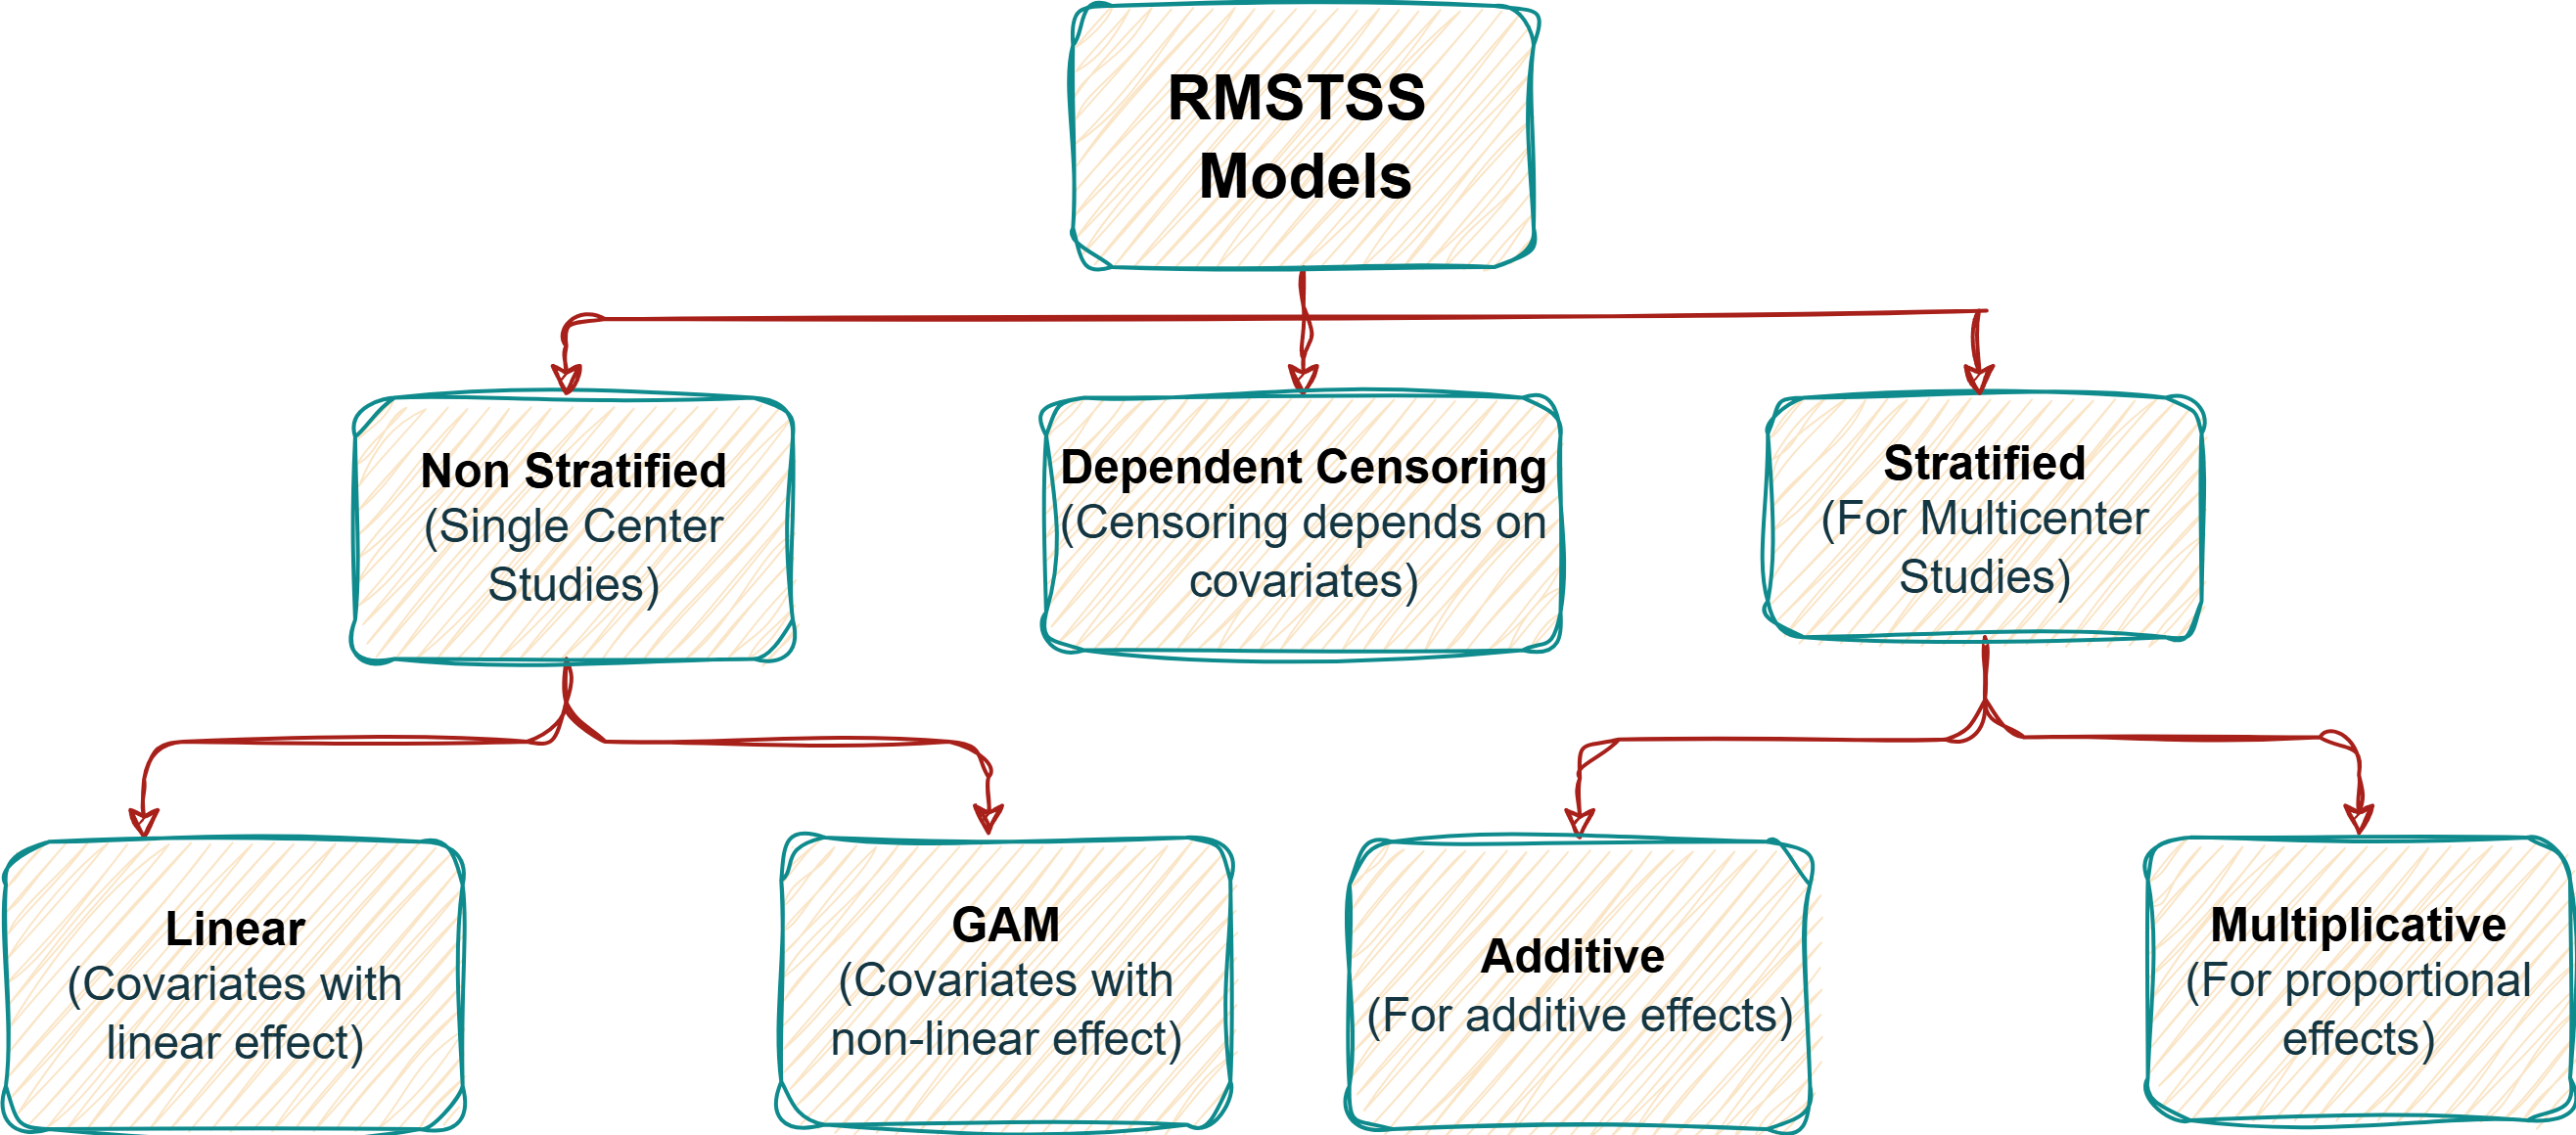
\includegraphics[width=1\linewidth]{images/app-models.png}
\end{figure}
\end{frame}


% --- Part 3: Non-Stratified Models ---

% ---------- Combined Slide: Notation + Linear Model ----------
\begin{frame}
\frametitle{Notation and Linear RMST Model}

\begin{block}{Observed Data}
For subject $i=1,\dots,n$:  
\begin{itemize}
  \item $Y_i = \min(T_i, C_i)$: observed follow-up time  
  \item $\delta_i = \mathbb{1}(T_i \le C_i)$: event indicator  
  \item $A_i \in \{0,1\}$: treatment group  
  \item $Z_i$: baseline covariates
\end{itemize}
\end{block}

\begin{block}{Linear RMST Model}
\[
E[\min(T_i,L) \mid A_i, Z_i] = \beta_0 + \beta_A A_i + \beta_Z^\top Z_i
\]

\begin{itemize}
  \item $\beta_A$: adjusted RMST difference between treatment arms  
  \item Direct regression not feasible due to censoring $\Rightarrow$ need IPCW
\end{itemize}
\end{block}

\end{frame}

% ---------- Frame 14 ----------
\begin{frame}
\frametitle{Simple Linear IPCW Model \citep{zhao2001}}

\begin{block}{Censoring Distribution}
Let $G(t) = P(C_i > t)$ be the survival function of censoring time.  
We estimate $\widehat{G}(t)$ using Kaplan–Meier.
\end{block}

\begin{block}{Weights}
Each subject receives weight
\[
w_i = \frac{\delta_i}{\widehat{G}(Y_i)}.
\]
\end{block}

\begin{block}{Weighted Least Squares}
Estimate $\beta$ by minimizing
\[
\widehat{\beta} = \arg\min_\beta \sum_{i=1}^n w_i \Big\{ Y_i - (\beta_0 + \beta_A A_i + \beta_Z^\top Z_i)\Big\}^2.
\]
\end{block}

\end{frame}

% ---------- Frame 15 ----------
% ---------- Combined Slide: Pseudo-Observations + GAM ----------
\begin{frame}
\frametitle{Generalized Additive Model \citep{parner2010}}

\begin{block}{Pseudo-Observations}
\[
\text{pseudo}_i(L) = n \cdot \widehat{\mu}(L) - (n-1)\cdot \widehat{\mu}^{(-i)}(L),
\]
\scriptsize
where $\widehat{\mu}(L)$ is the RMST estimate from the full sample and  
$\widehat{\mu}^{(-i)}(L)$ is the estimate with subject $i$ removed.  

\textbf{Key Property:}  
\[
E[\text{pseudo}_i(L)] = E[\min(T_i,L)]
\]
$\Rightarrow$ pseudo-observations can be treated as uncensored outcomes.
\end{block}

\begin{block}{Semiparametric GAM Model}
\[
E[\text{pseudo}_i(L)] = \beta_0 + \beta_A A_i + \sum_{k=1}^q f_k(Z_{ik}),
\]
\scriptsize
where $f_k(\cdot)$ are spline-based smooth functions.

\begin{itemize}
  \item $\beta_A$: adjusted RMST difference between treatment arms.  
  \item Handles censoring via pseudo-observations.  
  \item Captures nonlinear covariate effects flexibly while preserving interpretability.  
\end{itemize}
\end{block}

\end{frame}


% ---------- Frame 18 ----------
\begin{frame}
\frametitle{Stratified Models \citep{royston2011}}

\begin{block}{Additive Model}
Assume each stratum $j$ has its own baseline $\alpha_j$, with a common treatment effect:
\[
E[\min(T_i,L) \mid A_i, S_i=j] = \alpha_j + \beta_A A_i + \beta_Z^\top Z_i.
\]
Interpretation: $\beta_A$ is the constant added survival time across strata.
\end{block}

\begin{block}{Multiplicative Model}
Assume proportional treatment effect across strata:
\[
E[\min(T_i,L) \mid A_i, S_i=j] = \mu_{0j}(L) \cdot \exp(\beta_A A_i + \beta_Z^\top Z_i).
\]
Interpretation: $\exp(\beta_A)$ is the RMST ratio (treatment vs. control), common across strata.
\end{block}

\end{frame}

% ---------- Frame 17 ----------
\begin{frame}
\frametitle{Dependent Censoring \citep{robins2000}}

\begin{block}{Problem}
If censoring depends on covariates, a single $\widehat{G}(t)$ is biased.
\end{block}

\begin{block}{Solution: Cause-Specific Models}
For $K$ censoring causes, fit cause-specific hazards $\lambda_{Ck}(t \mid Z)$ and cumulative hazards $\Lambda_{Ck}(t \mid Z)$.  
Then
\[
\widehat{G}(t \mid Z) = \exp\!\Big(-\sum_{k=1}^K \widehat{\Lambda}_{Ck}(t \mid Z)\Big).
\]
\end{block}

\begin{block}{IPCW with Dependent Censoring}
Use $\widehat{G}(t \mid Z)$ in the IPCW weights.
\end{block}

\end{frame}

% --- Part 6: Software & Conclusion ---
% ---------- Frame 19 ----------
\begin{frame}
\frametitle{Power and Sample Size Calculation}

\begin{block}{Analytical Approach}
Uses asymptotic variance of the estimated treatment effect:
\[
\text{Power} = 
\Phi\!\left( 
\frac{|\widehat{\beta}_A|}{\widehat{\sigma}_{\beta_A}/\sqrt{n}} - z_{1-\alpha/2}
\right),
\]
where $\widehat{\sigma}_{\beta_A}$ is the estimated standard error and $\Phi$ is the standard normal CDF.
\end{block}

\begin{block}{Bootstrap Approach}
Simulation-based resampling from pilot data:
\[
\text{Power} =
\frac{\#\{\text{replicates with $p$-value} < \alpha\}}{B},
\]
where $B$ = number of bootstrap replicates.
\end{block}

\end{frame}

% ---------- Frame 21 ----------

\begin{frame}[fragile]{Example 1: Linear IPCW RMST Model}
\textbf{Goal:} Analytic sample size search for RMST difference under a linear IPCW model.

\begin{columns}[T,onlytextwidth]
  %%% LEFT: Code + notes %%%
  \begin{column}{0.55\textwidth}
  \scriptsize
    \begin{lstlisting}[language=R]
ss_results_vet <- linear.ss.analytical(
  pilot_data     = vet,
  time_var       = "time",
  status_var     = "status",
  arm_var        = "arm",
  target_power   = 0.40,
  linear_terms   = "karno",
  L              = 365,
  n_start        = 1000,
  n_step         = 250,
  max_n_per_arm  = 5000
)
    \end{lstlisting}
    {\scriptsize
    \textbf{Parameter Notes:} \\
    \texttt{n\_start} – starting sample size per arm . \\
    \texttt{n\_step} – increment in sample size at each step. \\
    \texttt{max\_n\_per\_arm} – upper cap on per‑arm sample size considered. \\
    }
  \end{column}

  %%% RIGHT: Figure + summary %%%
  \begin{column}{0.45\textwidth}
    \centering
    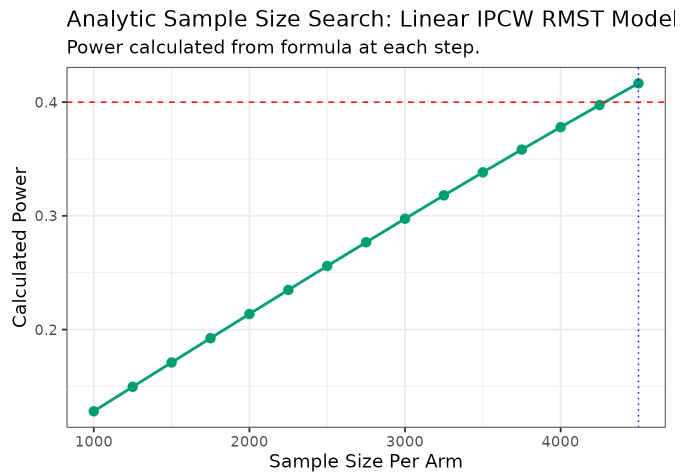
\includegraphics[width=\linewidth]{images/Example_LIN.png}

    \vspace{0.4em}
    \footnotesize
   \textbf{Simulation Summary}

    \vspace{0.25em}
 \begin{tabular}{@{}ll@{}}
      \toprule
      \texttt{Statistic} & \texttt{Value} \\
      \midrule
       RMST Difference  & -3.966558 \\
      \bottomrule
    \end{tabular}
  \end{column}
\end{columns}
\end{frame}


% ---------- Frame 22 ----------
\begin{frame}[fragile]{Example 2: Multiplicative Stratified RMST Model}
\textbf{Goal:} Estimate power for treatment effect on RMST ratio across strata using bootstrap.

\begin{columns}[T,onlytextwidth]
  %%% LEFT: Code %%%
  \begin{column}{0.6\textwidth}
  \scriptsize
    \begin{lstlisting}[language=R]
power_ms_boot <- MS.power.boot(
  pilot_data     = colon_death,
  time_var       = "time",
  status_var     = "status",
  arm_var        = "arm",
  strata_var     = "strata",
  sample_sizes   = c(100, 300, 500),
  L              = 1825,
  n_sim = 100, n_start = 100, n_step = 50,
  patience = 4, parallel.cores = 10
)
    \end{lstlisting}
    {\scriptsize
    \textbf{Parameter Notes:} \\
    \texttt{n\_sim} – \# bootstrap simulations. \\
    \texttt{n\_start} – initial sample size per stratum to evaluate. \\
    \texttt{n\_step} – increment in sample size during search. \\
    \texttt{patience} – \# iteration allowed w/o improvement. \\
    \texttt{parallel.cores} – \# cores to use for parallel processing.\\
    
    }
  \end{column}

  %%% RIGHT: Figure + table %%%
  \begin{column}{0.4\textwidth}
    \centering
    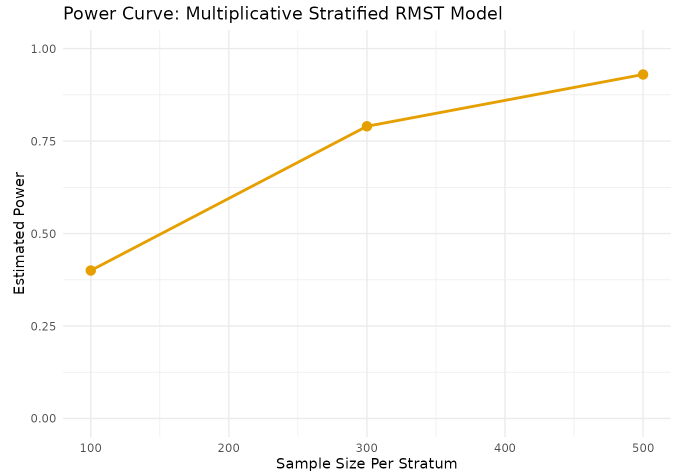
\includegraphics[width=\linewidth]{images/Example_MS.png}

    \vspace{0.4em}
    \footnotesize
    \textbf{Simulation Summary}

    \vspace{0.25em}
    \begin{tabular}{@{}ll@{}}
      \toprule
      Statistic        & Value \\
      \midrule
      Mean RMST Ratio  & 1.0065 \\
      95\% CI Lower    & 0.9680 \\
      95\% CI Upper    & 1.0572 \\
      \bottomrule
    \end{tabular}
  \end{column}
\end{columns}
\end{frame}



\begin{frame}
\frametitle{Application Interface}
\begin{figure}
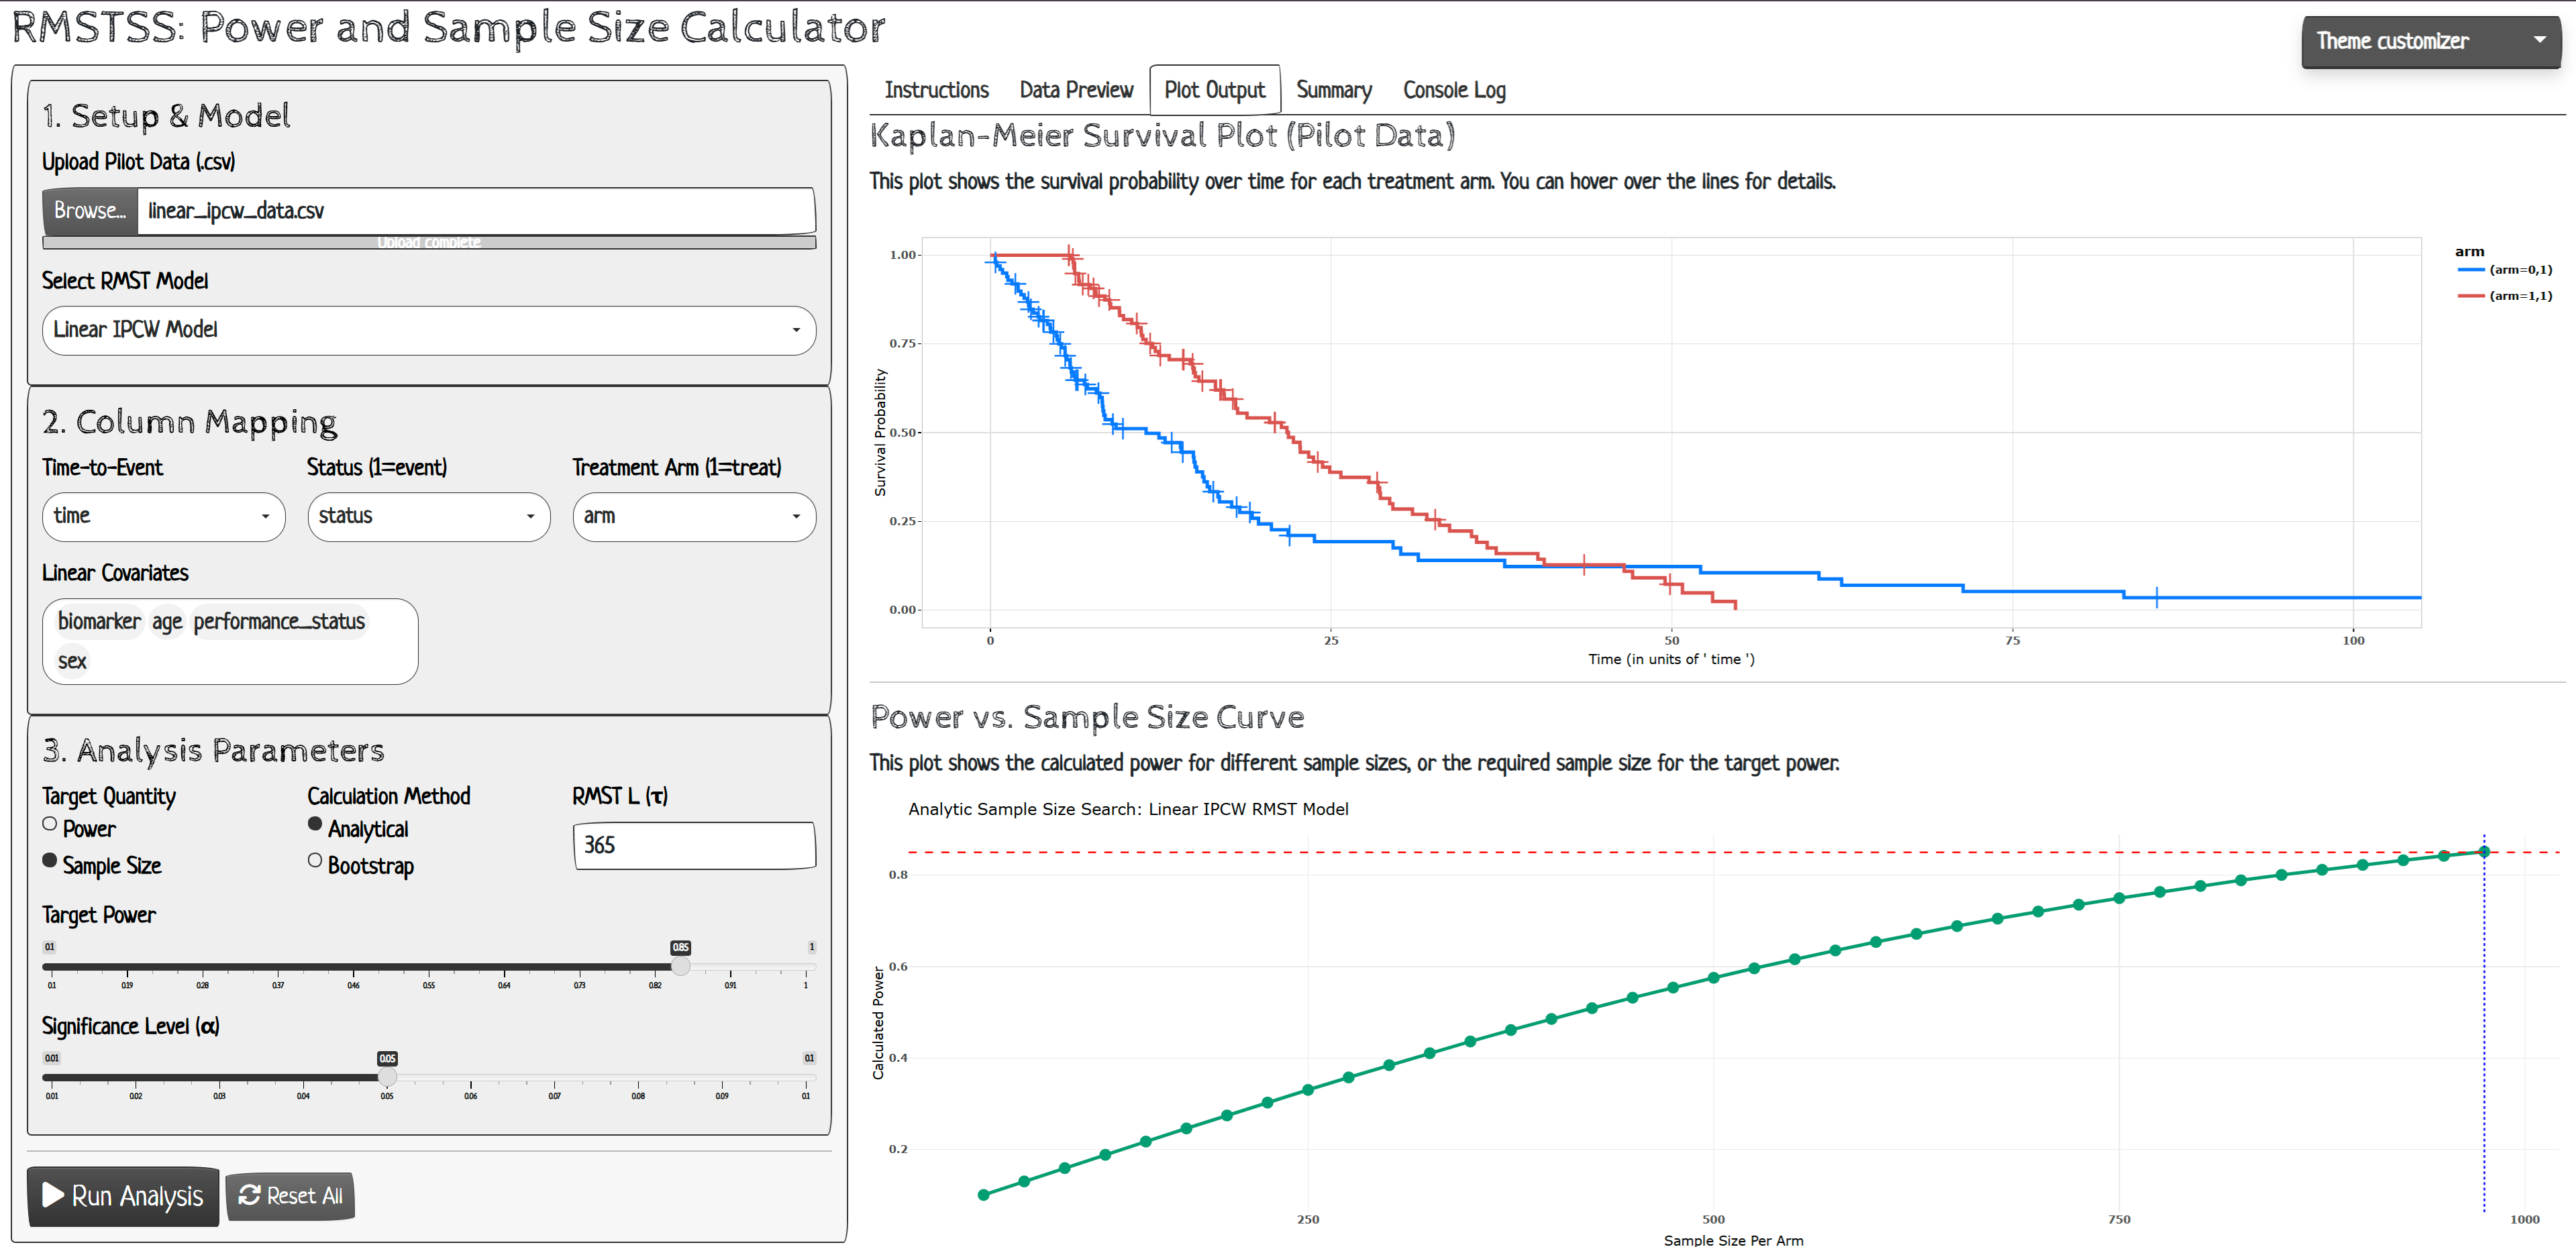
\includegraphics[width=\textwidth, height = 0.65\textwidth]{images/app-ss.png}
\end{figure}
\end{frame}
% ---------- Application Feature: vertical 3-step flow (arrows on bubbles) ----------
\begin{frame}
\frametitle{RMSTSS: Web Application Feature}

\centering
\scalebox{0.8}{%
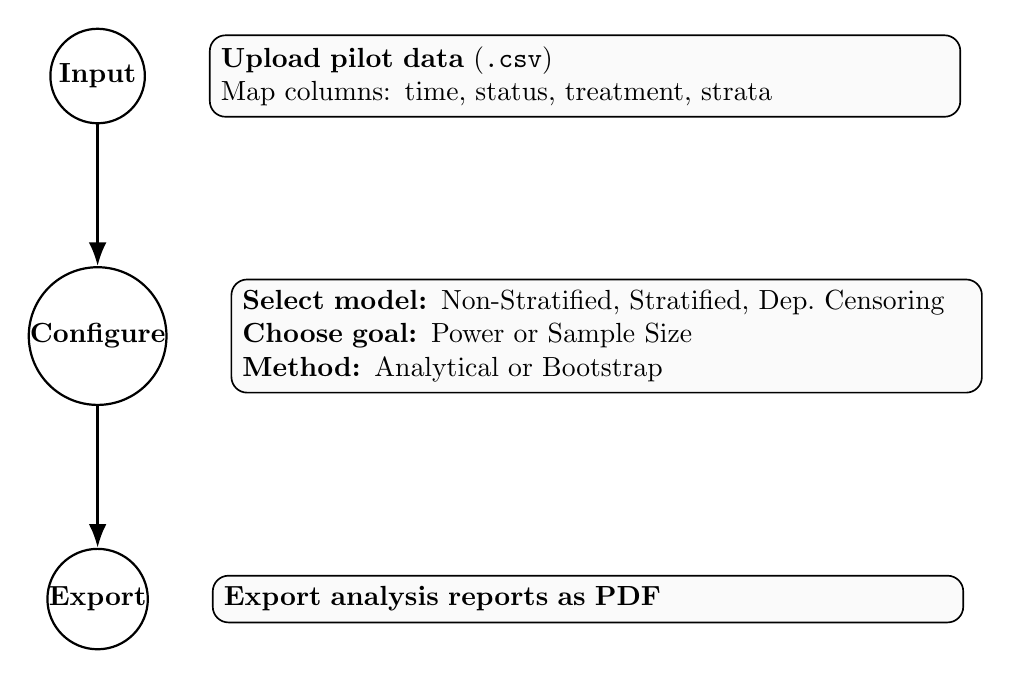
\begin{tikzpicture}[
  node distance=10mm and 8mm,
  bubble/.style={
    circle, draw, line width=0.8pt,
    minimum size=12mm, inner sep=0pt, font=\bfseries
  },
  box/.style={
    rectangle, rounded corners=2mm, draw, line width=0.6pt,
    align=left, inner sep=4pt, text width=9.25cm, fill=black!2
  },
  arr/.style={-{Latex[length=3mm]}, line width=1.pt}
]

% ===== Row 1: Input =====
\node[bubble] (b1) {Input};
\node[box, right=8mm of b1] (bx1) {%
  \textbf{Upload pilot data} (\texttt{.csv})\\
  Map columns: time, status, treatment, strata
};

% ===== Row 2: Configure =====
\node[bubble, below=18mm of b1] (b2) {Configure};
\node[box, right=8mm of b2] (bx2) {%
  \textbf{Select model:} Non-Stratified, Stratified, Dep.\ Censoring\\
  \textbf{Choose goal:} Power or Sample Size \\
  \textbf{Method:} Analytical or Bootstrap
};

% ===== Row 3: Export =====
\node[bubble, below=18mm of b2] (b3) {Export};
\node[box, right=8mm of b3] (bx3) {%
  \textbf{Export analysis reports as PDF}
};

% ===== Arrows between bubbles =====
\draw[arr] (b1.south) -- (b2.north);
\draw[arr] (b2.south) -- (b3.north);

\end{tikzpicture}%
}

\begin{itemize}
\centering
    \item \textbf{Fully web-based} — no R installation required
    \item \textbf{Interactive} plots and \textbf{customizable} visual environment
\end{itemize}
\end{frame}





% ---------- Frame 24 ----------
\begin{frame}
\frametitle{Conclusion \& Future Aims}

\begin{block}{Conclusion}
\begin{itemize}
  \item \textbf{Statistically Rigorous:} Implements linear, GAM, dependent censoring, and stratified RMST models
  \item \textbf{Causally Interpretable:} Treatment effect $\beta_A$ (difference) or $\exp(\beta_A)$ (ratio)
  \item \textbf{Practical:} Available as both an R package and a Shiny web app
\end{itemize}
\end{block}

\begin{block}{Future Aims}
\begin{itemize}
  \item Extend RMSTSS to handle time-varying treatments
  \item Incorporate data-generating mechanism to avoid pilot data
  \item Develop modules for multi-arm and platform trials
\end{itemize}
\end{block}
\end{frame}


% Frame 25: Access & Acknowledgments
\begin{frame}
\frametitle{Access \& Acknowledgments}
\begin{columns}[T]
\begin{column}{0.5\textwidth}
\scriptsize
    \textbf{Acknowledgments}
 \begin{itemize}
        \item Grateful appreciation to Dr.\ Yuan Zhang (UTHSC) for mentorship
        \item Special thanks to Dr.\ Gregory Farage and Dr.\ Saunak Sen (UTHSC) for their guidance and support
        \item Support provided by UTHSC BERD (Biostatistics, Epidemiology, and Research Design)
        \item Research funded by NSF Grant No.\ 2220726
    \end{itemize}
\vfill
\begin{center}
\Huge{\textbf{Questions?}}
\end{center}
\end{column}
    \begin{column}{0.5\textwidth}
    \scriptsize
        \centering
        \textbf{Scan for Web App} \\
        \qrcode[height=3cm]{https://arnab96.shinyapps.io/uthsc-app/}
        \vspace{2em}
        \\
        \textbf{Scan for R Package} \\
        \qrcode[height=3cm]{https://uthsc-zhang.github.io/RMSTSS-Package/}
    \end{column}
\end{columns}
\end{frame}

\begin{frame}
\frametitle{References}
\scriptsize
\bibliographystyle{plainnat}
\bibliography{references}
\end{frame}

\end{document}
